\section{Classroom Settings}\label{classroom-study-settings}

The setting for this study was an undergraduate course in an intelligence
training program at Pennsylvania State University. The program was designed to train students
to become professional intelligence analysts. A key requirement of the course is
to emphasize hands-on practice on team-based intelligence analysis.

 %\bvh{I would make a bigger point about the training in the tools that they
 %already had, they were sort of primed to not use a collaborative tool}

 % \bvh{separate the argument about waterfall and what students were already trained in and how it played out}
 During the first ten weeks of the course
 students learned several analytic techniques, including IEW (a technique
 to extract evidence and assess their values), ACH (a technique to evaluate
 multiple hypotheses against evidence), timeline analysis and network
 analysis, as well as state-of-the-art tools to implement these
 techniques, including Analyst's Notebook and PARC ACH. Students also practiced applying these
 techniques in two hands-on projects before our study. Students follow a typical ``waterfall'' workflow: they start with IEW to
 extract evidence from documents and model them into a structured format. With that data available, they start building analytic
 artifacts such as an ACH Matrix in PARC ACH, and a timeline and a network
 graph in Analyst's Notebook. Sometimes the process is not necessarily sequential, and they want to jump back to edit data when building analysis. Yet since the tools are separate and data within the tools are not sharable, the annotation activity and analysis activity are largely isolated and streamlined. 
 
 Most tools in use lack serious collaboration
 support (except that some teams use Google Doc to construct an IEW
 table). Analysts were unable to contribute simultaneously, an issue
 known as production blocking \citep{Diehl1987a}. Students often divide their work by tools: each person picks a tool, creates and analyzes an artifact
 with that tool on their own, and puts individual analysis together towards the end. This had the consequence that findings and
 hypotheses were made without integrating collective efforts and diverse
 knowledge. Analysts coordinated work by manually sharing documents
 or graphs through email or cloud storage service (e.g.~Dropbox),
 resulting in a scattered placement of results, requiring repeated manual
 resynchronizing to identify redundant or missing pieces of information,
 analysis of information, and analytic hypotheses. In summary, the students in our study had learned and practiced with tools lack of support for collaboration and were all aware of the shortcomings.

 %\bvh{do demographic stuff first}
 Of the 98 students enrolled in the course (from
 two sections), 73 consented to participate in the study. All of the 73 students
 majored in the program of Security and Risk Analysis. Most (75\%) of them
 were in the third academic year ($M=3.06 \text{ years}, SD=.44$), indicating that participants in
 our study had relatively advanced experience and knowledge in intelligence
 analysis. Participants' age ranged from 19 to 28 ($M=20.4, SD=1.18$). 77\% of the
 participants were male.

 Students were given a tutorial on CAnalytics a week before the project began.
 One of the authors walked through the features of CAnalytics, without enforcing or implying any strategic use of the tool. Students then accomplished a small case analysis at their own pace. During the week of the
 actual study, one author was constantly available to help with any technical
 issues. Although students were encouraged to make full use of CAnalytics, to
 ensure a natural environment students were always free to employ any other
 tools that they believed useful.

 \begin{figure}
 	\centering
 	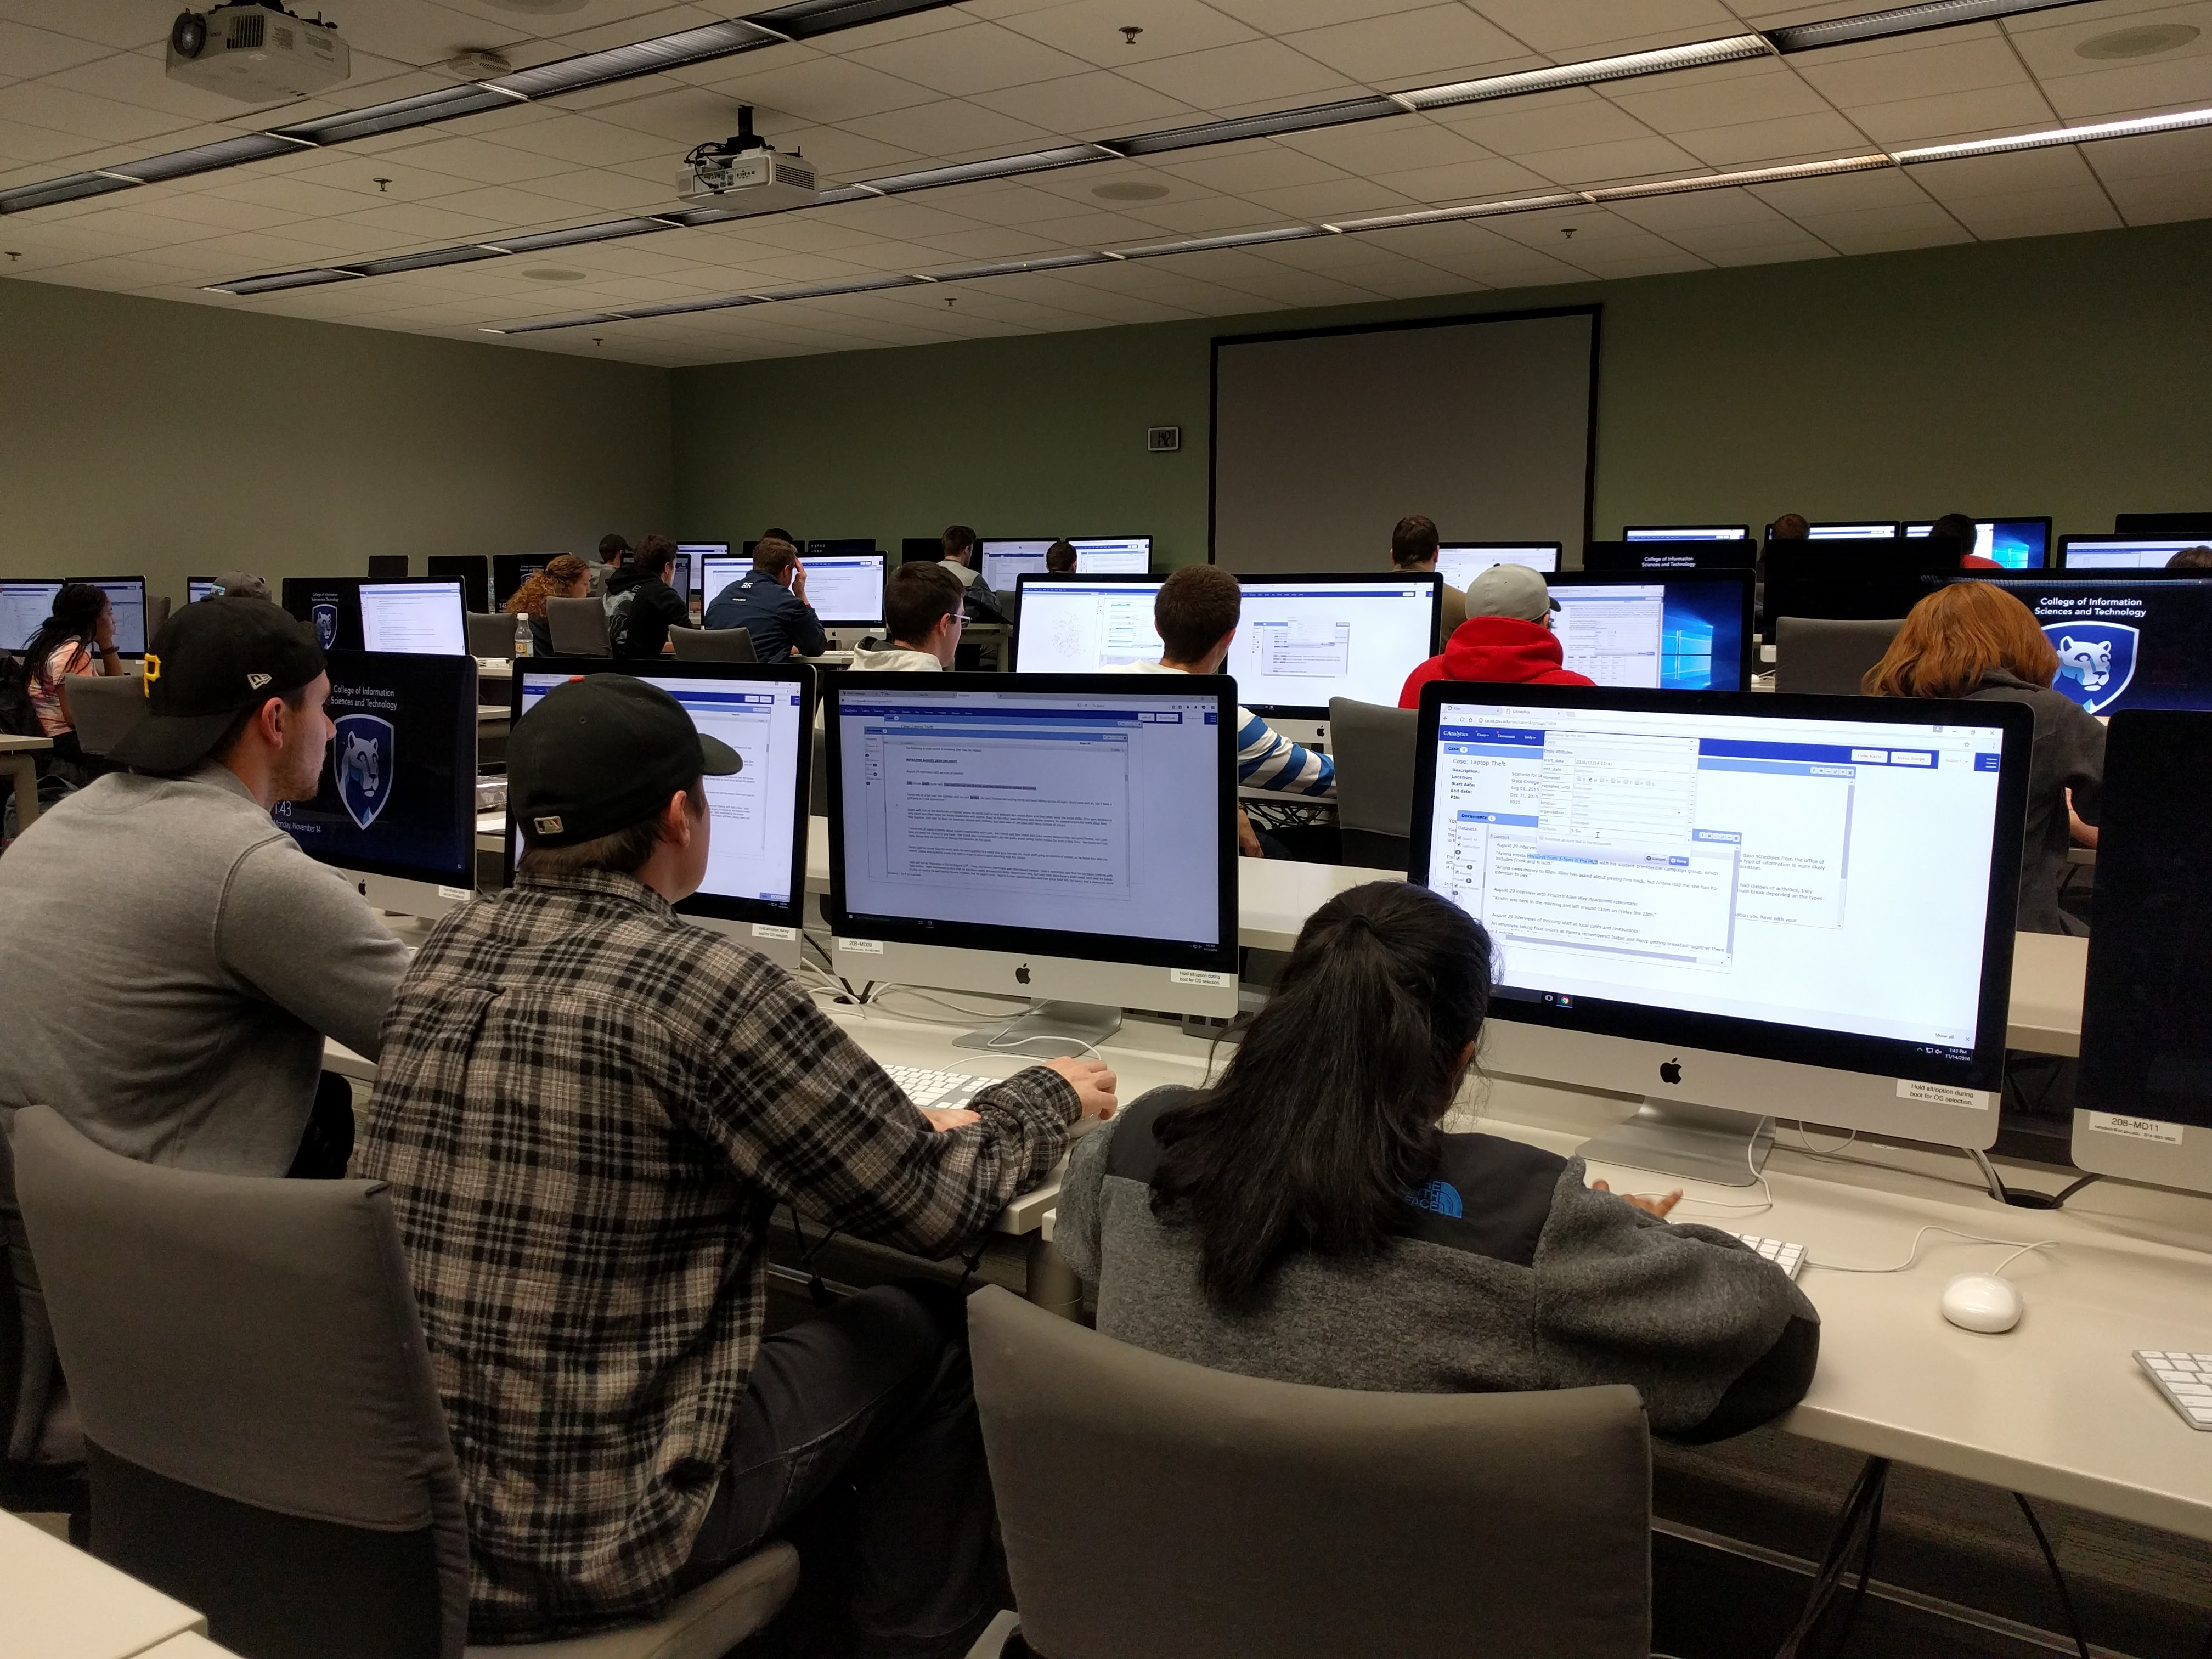
\includegraphics[width=3in]{04-Study_one/img/classroom_setting.jpg}
  \caption{Classroom setting}\label{fig:classroom}
 \end{figure}

Our study began on the 10th week of the course and lasted for one week. The
analysis that students performed on our tool was an investigation of a series
of bank robberies. The case and materials were fabricated by the course instructor. Teams
were provided a set of documents pertaining to seven robberies, including police
reports, witnesses reports, video records, and news media. The analysis was
designed to be open-ended, meaning that there was no single, definitive answer.
The instructor explained that the task was to simulate real world scenarios, in
which analysts always reasoned in the circumstances of uncertainty, ambiguity,
and complexity. The instructor told the students that he expected the analysis
to take around 6 hours, including in-class and outside-class work. At the end of
the project students were required to submit a team report, describing their
hypotheses, assumptions, conclusions, and supporting evidence. When in class, students used a 27-in Macintosh desktop (as shown in Figure~\ref{fig:classroom}. Students could use any equipment when outside class.

Students were randomly assigned into 25 teams (23 three-person teams and 2
two-person teams). Research suggests that group size is an important factor in
group collaboration, and two-person teams might behave differently from
three-person teams. We thus excluded data from the two-person teams in our
analysis in this paper. Also, from the log (and confirmed by their
questionnaire), we found that one team made little use of CAnalytics and opted
for other tools (Google Doc). Hence their data were also excluded. Our final data report includes the result from 22 teams.

\section{Data collection and analysis}

We employed several data collection approaches. We administrated a post-study
questionnaire (Appendix E). The questions used a 7-point likert scale and included 7 items measuring an individual's
self-reported awareness, 7 items for
communication quality, 6 items for collective efficacy, and 3 items for perceived performance \citep{Convertino2011}. We also used NASA-TLX \citep{Hart1988} to measure cognitive load. The questionnaire
also included open-ended questions asking how the tool helped or impeded their
work. 

We captured user interactions with system logs. Instead of simply logging
low-level events like mouse clicks and keyboard strokes, we recorded meaningful actions such
as creating an annotation and deleting an entity. The full log schema is listed in Section~\ref{activity-og}.  

Finally, we reviewed team
reports and graded them as an indicator of team performance. Since the task was
open-ended, there was no single right answer. We constructed an assessment
rubric together with the course instructor by listing all possible hypotheses
and evidence from the documents, with a full score of 16. I and another researcher graded the reports independently. If the grades differ by
less than 2, an average is set as the final grade (14 out of 22 reports).
Otherwise (the rest 8 reports), the two graders review the reports together and
make an agreement.

Multiple methods were used to analyze the collected data. We analyzed the artifacts (visualizations and annotations) people created. The premise is that artifacts teams create to support their work activity can be a window into their cognitive and collaborative process \citep{Carroll2013}. Since all user data is stored in the system, we could restore user-created artifacts and compare the differences across teams. We also pulled user's interaction logs and visualized them in sequence, in an attempt to identify patterns within a team and across teams.

We did qualitative analysis over answers from the open-ended questions. We employed an open coding approach in development of our coding schema. We iteratively went through the data and added emerging themes to the schema. The believability of the result is achieved by data triangulation among user logs and their created artifacts. Each interpretation is followed by users’ quoted comments. The repeatedly identified themes guarantee believable interpretation output in the study. 

Finally, we did statistic analysis over survey scales and team performance (as measured by report grades). The analysis attempted to capture factors that account for team performance variance quantitatively. The result is reported below.
